\documentclass[a4paper,12pt]{article} 

%%%%%%%%%%%%%%%%%%%%%%%%%%%%%%%%%%%%%%%%%%%%%%%%%%%%%%%%%%%%%%%%%%%%%%%%%%%%
\usepackage[utf8]{inputenc}
\usepackage[spanish]{babel}
\usepackage{amsmath}
\usepackage{amsfonts}
\usepackage{amssymb} 
\usepackage{graphicx} 
\usepackage{hyperref} 
\usepackage{wrapfig}
\usepackage{enumitem}
\usepackage{blindtext}
\usepackage{fancyhdr}
\usepackage{float}
\usepackage{eurosym}
\usepackage{color}
\usepackage{titling}
\usepackage{amssymb, amsmath, amsbsy} % simbolitos
 \usepackage{upgreek} % para poner letras griegas sin cursiva
 \usepackage{cancel} % para tachar
 \usepackage{mathdots} % para el comando \iddots
 \usepackage{mathrsfs} % para formato de letra
\usepackage{stackrel} % para el comando \stackbin
\usepackage{lipsum}
\usepackage{tocbibind}
\usepackage[T1]{fontenc}
\usepackage[left=3cm,right=3cm,top=3cm,bottom=4cm]{geometry}
\pagestyle{fancy}
%%%%%%%%%%%%%%%%%%%%%% CABECERAS %%%%%%%%%%%%%%%%%%%%%%%%%%%%%%%%%%%%%%%%%%%
\newcommand{\hsp}{\hspace{20pt}}
\newcommand{\HRule}{\rule{\linewidth}{0.5mm}}
\headheight=50pt
\newcommand{\vacio}{\textcolor{white}{holacaracola}}
%%% NUMERACION DE ECUACIONES
\renewcommand{\theequation}{\thesection.\arabic{equation}}
% COLOR AZUL PARA TEXTOS EN PORTADA
\definecolor{azulportada}{rgb}{0.16, 0.32, 0.75}
% Azul para textos de headings
\definecolor{azulinterior}{rgb}{0.0, 0.2, 0.6}

%%%%%%%%%%%%%%%%%%% DATOS DEL PROYECTO %%%%%%%%%%%%%%%%%%%%%%%%%%%%%%%%%%%%%
\title{Actividad 7}
\author{}
\newcommand{\director}{Carlos Lizárraga Celaya}

\begin{document}
\begin{titlepage}
\begin{center}
\vspace{1cm}

\includegraphics[width=5.5cm]{unison-logo.png}
\\[0.5cm]
{\fontfamily{phv}\fontsize{24}{6}\selectfont{UNIVERSIDAD DE SONORA}}\\
[1em]
{\fontfamily{phv}\fontsize{16}{5}\selectfont{DEPARTAMENTO DE FÍSICA}}\\
[4em]
\textcolor{azulportada}
{\fontfamily{phv}\fontsize{30}{5}\selectfont{\textsc{\thetitle}}}\\
% Autor del trabajo de investigación
[1cm]
{\fontfamily{phv}\fontsize{16}{5}\selectfont{Alumno:}}\\
[0.2cm]
%Equipo sfdsfshkfhsfhsjfs
{\fontfamily{phv}\fontsize{14}{5}\selectfont{Luis Alfonso Torres Flores}}\\
[1cm]
%{\Huge\textbf{\thetitle}}\\
{\fontfamily{phv}\fontsize{16}{5}\selectfont{Profesor}}\\
[0.2cm]
{\fontfamily{phv}\fontsize{16}{5}\selectfont{\director}}\\
[4.5cm]
{\fontfamily{phv}\fontsize{14}{5}\selectfont{18 de Abril de 2017}}\\
[4cm]
\end{center}
\restoregeometry
\end{titlepage}

\newpage
%%%Encabezamiento y pie de página
\renewcommand{\headrulewidth}{0.5pt}
\fancyhead[R]{
	\textcolor{azulinterior}{\fontfamily{phv}\fontsize{14}{4}\selectfont{\textbf{\thetitle}}}\\
\textcolor{azulportada}{\fontfamily{phv}\fontsize{10}{3}\selectfont{Curso de Fisica computacional}}\\
{\fontfamily{phv}\fontsize{10}{3}\selectfont{\theauthor}}}
\fancyhead[L]{\vacio}

\newpage
\tableofcontents
\newpage
%------------------------------
\section{Breve resumen}
\noindent
En la anterior actividad se utilizó la transformada discreta de Fourier, quitándole a las olas sus fases y obteniendo como resultado la gráfica respectiva a ese trabajo, ahora iremos de atrás para delante y buscaremos obtener la gráfica inicial que se obtiene haciendo uso de los datos.
%------------------------------
\section{Introducción}
\noindent
Hasta el momento hemos trabajado con las mareas de Baltimore, Maryland y Topolobampo, Sinaloa. Usamos datos de los meses de enero, febrero y marzo del año 2016. Debido a la naturaleza del trabajo, este se realizó encima del código de la actividad 6, pues esta actividad es una regresión a la gráfica original. Nos encontramos con un problema aquí, si bien podemos utilizar una función donde simplemente podríamos ingresar una amplitud y el coseno del producto de nuestro periodo, nuestra frecuencia y un valor t, pero hay algo que se llegó a omitir, la fase. En la actividad 6, gracias al código empleado ahí, quitamos la fase, borramos ese factor que nos decía en que determinados tiempos volvería a aparecer dicha marea, por lo que el principal problema es encontrar esa fase. Se usaron datos de la actividad 6, como viene siendo la hora en la que ocurren los principales puntos de las mareas, esos picos representativos de nuestra grafica de la transformada de Fourier que nos ayudaran a realizar la regresión. Si nos damos cuenta, esta actividad puede cerrar un circulo con la actividad anterior, puesto que llegamos a un punto con la transformada de Fourier y ahora nos estamos regresando al inicio con la mayor precisión posible.
%------------------------------
\section{Procedimiento}
\noindent
Después de la transformada de Fourier nosotros ya habíamos pedido que se nos dieran las alturas superiores a un valor y con esto la hora o número de dato que le corresponde. Nosotros necesitamos las amplitudes representativas, sus frecuencias y su fase correspondiente. Ya tenemos los nodos identificados, solo nos quedaríamos con las horas en las que ocurren, con lo que usaríamos el código que se menciona en sus correspondientes apartados para cada uno de los lugares. Si bien notamos solo hacemos referencia a dichos datos de las horas, toando 12 datos en caso de Baltimore ignorando al cero y 4 en el caso de Topolobampo, puesto que su grafica con la transformada de Fourier se puede notar que no tiene muchas alturas representativas. 

La frecuencia fue lo que se buscó de forma consecutiva, como bien notaremos abajo se sumó un valor 1092 a todas ellas, esto se debe a que solo estamos buscando datos del lado derecho de la gráfica, valores positivos del eje X, por lo que al sumarle dicho valor junto con el dato obtendríamos la frecuencia que observamos en la gráfica.

Por último, tenemos la fase, el mayor problema que se presentó en esta actividad. La fase se buscó en forma de un ángulo para su posterior coloca miento en la función empleada en este trabajo. Dicha función tiene un formato de $(Amplitud)*cos(Periodo*Frecuencia*fase) $, que como bien utilizamos distintas amplitudes representativas, tenemos una sumatoria de cosenos con sus respectivas amplitudes, frecuencias y fases. Las cuales se graficaron y podremos observar. Se colocó en color azul la gráfica que se obtiene directamente con los datos descargados de las paginas oficiales de sus correspondientes lugares y en rojo la gráfica obtenida con este procedimiento.


\subsection{Baltimore}
\subsubsection{Código de amplitud}
\noindent
$A0_m = np.absolute(yf[0]/N)$\\
$O1_m = np.absolute(yf[4]/N$\\
$S1_m = np.absolute(yf[6]/N)$\\
$N2_m = np.absolute(yf[7]/N)$\\
$M2_m = np.absolute(yf[11]/N)$\\
$Q2_m = np.absolute(yf[12]/N)$\\
$F2_m = np.absolute(yf[14]/N)$\\
$S2_m = np.absolute(yf[18]/N)$\\
$D2_m = np.absolute(yf[24]/N)$\\
$G2_m = np.absolute(yf[29]/N)$\\
$H2_m = np.absolute(yf[30]/N)$\\
$J2_m = np.absolute(yf[44]/N)$\\
$K2_m =np.absolute(yf[176]/N)$

\subsubsection{Código de frecuencia}
\noindent
$T_S1 =  xf[int(1092 +4),]$\\
$T_N2 =  xf[int(1092 +6),]$\\
$T_M2 =  xf[int(1092 +7),]$\\
$T_S2 =  xf[int(1092 +11),]$\\
$T_Q2 =  xf[int(1092+12)]$\\
$T_R2 =  xf[int(1092+14)]$\\
$T_T2 =  xf[int(1092+18)]$\\
$T_Y2 =  xf[int(1092+24)]$\\
$T_U2 =  xf[int(1092+29)]$\\
$T_I2 =  xf[int(1092+30)]$\\
$T_O2 =  xf[int(1092+44)]$\\
$T_P2 =  xf[int(1092+176)]$\\

\subsubsection{Código de fase}
\noindent
$T_S1s =np.angle(yf[int(4),])$\\
$T_N2s =np.angle(yf[int(6),])$\\
$T_M2s =np.angle(yf[int(7),])$\\
$T_S2s=np.angle(yf[int(11),])$\\
$T_Q2s = np.angle(yf[int(12)])$\\
$T_R2s =np.angle(yf[int(14)])$\\
$T_T2s =np.angle(yf[int(18)])$\\
$T_Y2s =np.angle(yf[int(24)])$\\
$T_U2s =np.angle(yf[int(29)])$\\
$T_I2s =np.angle(yf[int(30)])$\\
$T_O2s =np.angle(yf[int(44)])$\\
$T_P2s =np.angle(yf[int(176)])$\\

\subsubsection{Función}
\noindent
$y= df['Altura']$\\
$w= 2.0*np.pi$\\

def $f(t):$\\
    return $ A0_m + 2*(O1_m*np.cos(w *T_S1*t+T_S1s) + S1_m*np.cos(w*T_N2*t+T_N2s)
+ N2_m*np.cos(w*T_M2*t+T_M2s) +M2_m*np.cos(w*T_S2*t+T_S2s) +Q2_m*np.cos(w*T_Q2*t+T_Q2s)               +F2_m*np.cos(w*T_R2*t+T_R2s) +S2_m*np.cos(w*T_T2*t+T_T2s)+D2_m*np.cos(w*T_Y2*t+T_Y2s)                +G2_m*np.cos(w*T_U2*t+T_U2s)+H2_m*np.cos(w*T_I2*t+T_I2s)+J2_m*np.cos(w*T_O2*t+T_O2s)                   +K2_m*np.cos(w*T_P2*t+T_P2s))$

\subsubsection{Gráfica}

\begin{center}
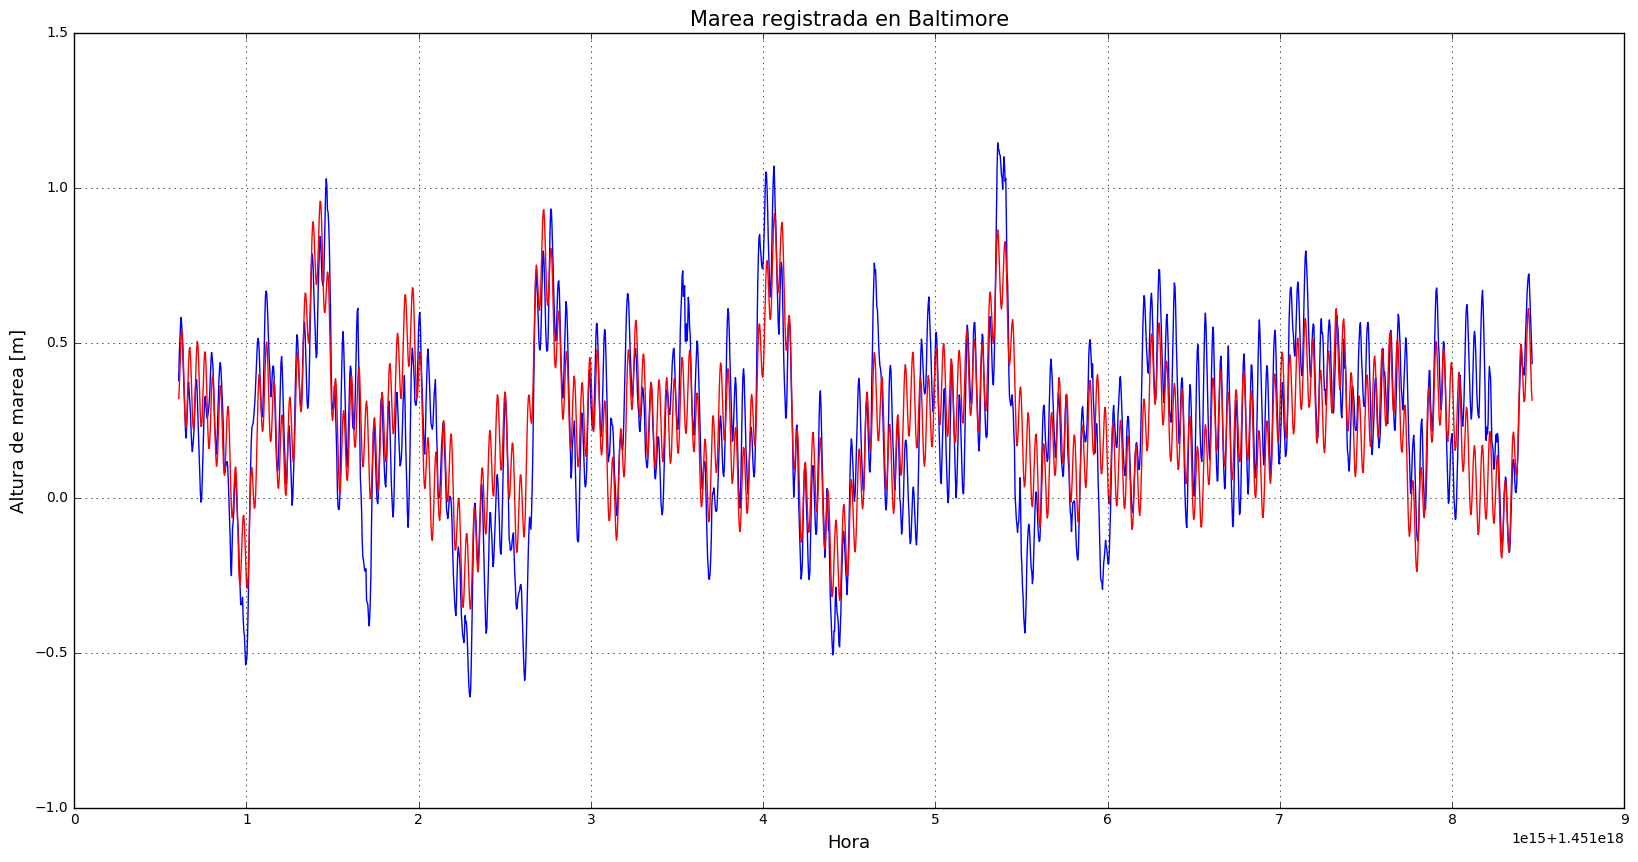
\includegraphics[scale=0.4]{graficabalti7.png}
\end{center}


%-----------------------------
\subsection{Topolobampo}
\subsubsection{Código de amplitud}
\noindent
$A0_m = np.absolute(yf[0]/N)$\\
$O1_m = np.absolute(yf[85]/N)$\\
$S1_m = np.absolute(yf[91]/N)$\\
$N2_m = np.absolute(yf[176]/N)$\\
$M2_m = np.absolute(yf[182]/N)$

\subsubsection{Código de frecuencia}
\noindent
$f_O1 = yf[int(1092)]$\\
$T_S1 = xf[int(1092+85),]$\\
$T_N2 = xf[int(1092+91),]$\\
$T_M2 = xf[int(1092+176),]$\\
$T_S2 = xf[int(1092+182),]$

\subsubsection{Código de fase}
\noindent
$f_O1s = np.angle(yf[int(1092)])$\\
$T_S1s = np.angle(yf[int(85),])$\\
$T_N2s = np.angle(yf[int(91),])$\\
$T_M2s = np.angle(yf[int(176),])$\\
$T_S2s = np.angle(yf[int(182),])$

\subsubsection{Función}
\noindent
$y= df['Altura']$
$w= 2.0*np.pi$

def $f(t):$\\
    return $A0_m + 2*(O1_m*np.cos(w*T_S1*t+T_S1s) + S1_m*np.cos(w * T_N2 *t+T_N2s) + N2_m*np.cos(w*T_M2*t+T_M2s) 
+ M2_m*np.cos(w*T_S2*t+T_S2s))$

\newpage
\subsubsection{Gráfica}

\begin{center}
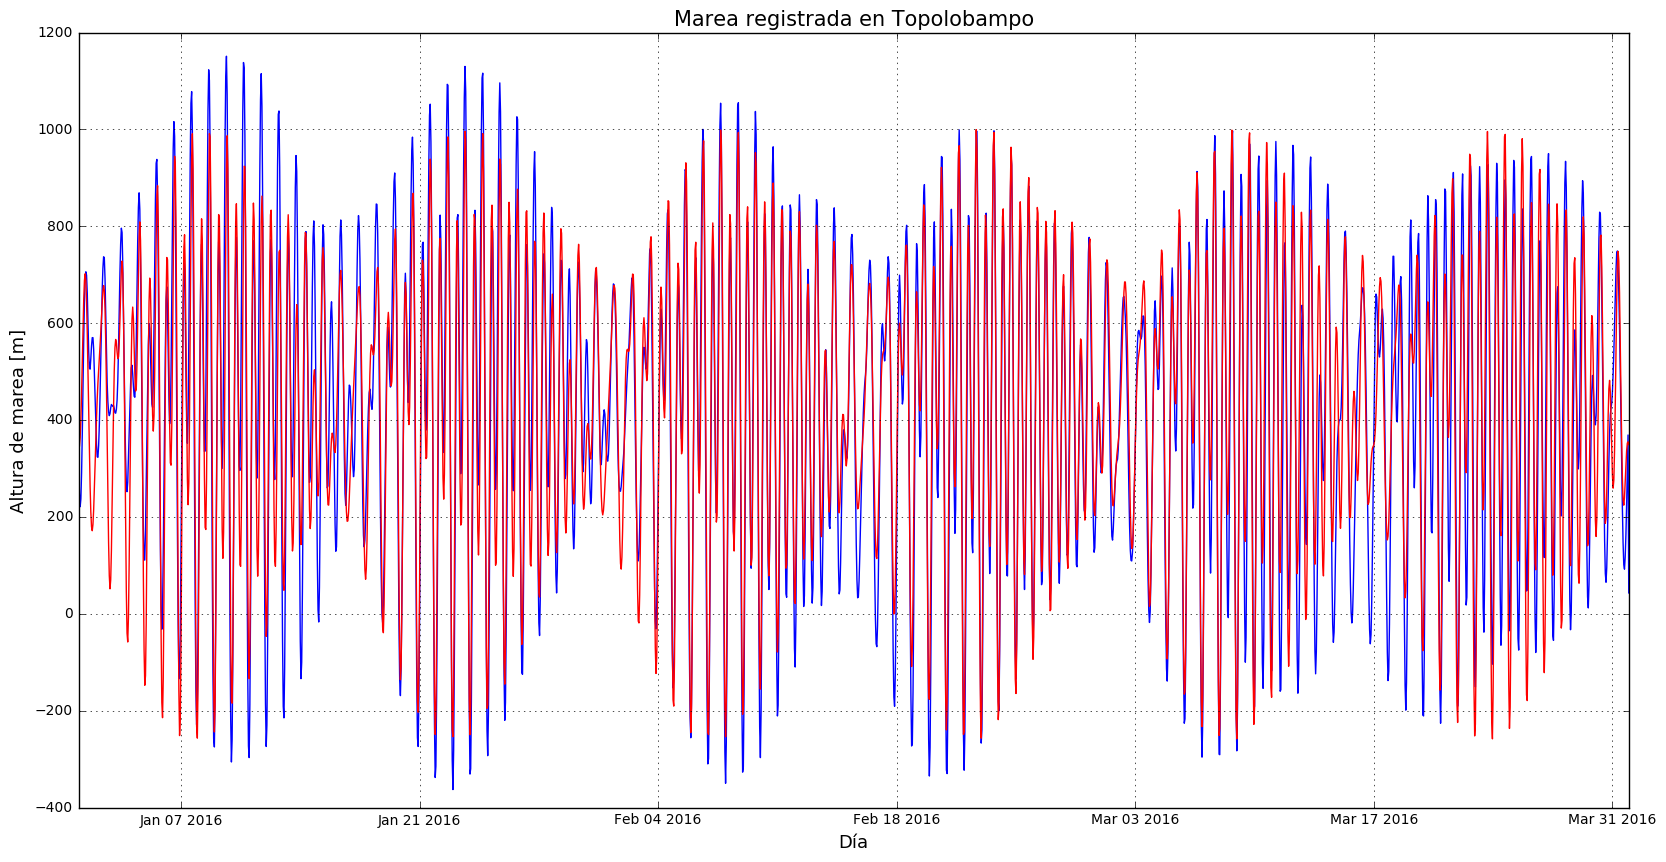
\includegraphics[scale=0.4]{graficatopo7.png}
\end{center}
%------------------------------
\section{Error relativo}
\noindent
Se calculó el error relativo respecto a la gráfica original y la gráfica obtenida mediante el anterior procedimiento. Se mostrará el código y una tabla con sus errores de las mareas de los lugares estudiados.
\subsection{Código}
\noindent
$y_0 = df['Altura']$\\
$y_1 = f(df['T'])$\\
\noindent
$E= sum(abs(y_0-y_1)**2) / sum(abs(y_0)**2)$\\
E

\centering
\begin{tabular}{|c|c|}
\hline
Lugar & Error relativo \\ \hline
Baltimore & 23.92 \% \\ \hline
Topolobampo & 6.24\% \\ \hline
\end{tabular}
\end{document}
